\documentclass{article}

% PREAMBLE: This section defines the document's overall style and includes necessary packages.

% The 'geometry' package allows for easy customization of page margins and layout.
% Here, we set 1-inch margins on all sides and a text width of 6.5 inches.
\usepackage[margin=1in, textwidth=6.5in]{geometry}

% The 'graphicx' package is essential for including images.
\usepackage{graphicx}

% AMS packages provide extended environments and features for mathematics.
\usepackage{amsmath}    % For advanced math environments like 'align*'
\usepackage{amssymb}    % For additional math symbols
\usepackage{amsfonts}   % For math fonts

% The 'enumitem' package provides control over list environments (itemize, enumerate).
\usepackage{enumitem}

% The 'pdfpages' package allows for the inclusion of external PDF documents.
\usepackage{pdfpages}

% --- Document Title ---
% We create a title for the study guide. The author and date are left blank as requested.
\title{Chapter 8 Quiz - Revision}
\author{}
\date{}

\begin{document}

\maketitle % This command generates the title based on the \title, \author, and \date commands.

% ---------------------------------------------------------------------------------------------------
% SECTION 1: QUIZ DETAILS AND TOPICS
% ---------------------------------------------------------------------------------------------------
\hrulefill
\subsection*{Quiz Details}
\begin{itemize}[itemsep=5pt] % 'itemsep=5pt' adds vertical space between list items for readability.
    \item \textbf{Date and Time:} Tuesday, September 30th, between 7:00 AM and 7:30 AM.
    \item \textbf{Format:} Closed notes.
    \item \textbf{Allowed Materials:} A clean, unmarked copy of the provided periodic table (``Periodic Table for testing.pdf''). Ensure there is no writing on it.
\end{itemize}
\hrulefill
\subsection*{Key Topics on the Quiz}
\begin{enumerate}[itemsep=5pt]
    \item Balancing chemical equations and identifying the type of reaction (synthesis, decomposition, single exchange, double exchange, combustion).
    \item Calculating the molecular formula from a given empirical formula and molar mass.
    \item Calculating the theoretical yield of a product when one reactant is explicitly stated to be in excess.
\end{enumerate}
\hrulefill
\bigskip % Adds a larger vertical space to separate major sections.

% ---------------------------------------------------------------------------------------------------
% SECTION 2: PHASED STUDY PLAN
% ---------------------------------------------------------------------------------------------------

\subsection*{Phase 1: Foundation \& Review (Friday - Saturday)}
\begin{itemize}[itemsep=5pt]
    \item \textbf{Understand Reaction Types:} Review slides 12-17 in \texttt{Chapter 8 Powerpoint.pdf}. Focus on the definitions and general forms (e.g., A + B $\rightarrow$ AB for synthesis) for each reaction type.
    \item \textbf{Master Balancing Equations:} Review slides 6-11 in \texttt{Chapter 8 Powerpoint.pdf}. Pay close attention to the strategy of balancing compounds first and treating polyatomic ions as single units.
    \item \textbf{Review Stoichiometry Concepts:} Refresh your understanding of mole-to-mole and gram-to-gram conversions by reviewing slides 25-31 in \texttt{Chapter 8 Powerpoint.pdf}. This is the foundation for theoretical yield problems.
\end{itemize}

\bigskip

\subsection*{Phase 2: Practice \& Application (Saturday - Sunday)}
\begin{itemize}[itemsep=5pt]
    \item \textbf{Practice Balancing and Classifying:} Complete problems 1a through 1l on the first page of \texttt{Types of Chemical Reactions.pdf}. Check your answers against the solutions provided on the sheet. For extra practice, work through problems 6a, 6b, 6c, and 6e on page 4.
    \item \textbf{Practice Theoretical Yield:} Work through problem 4 from \texttt{Limiting Reagent Worksheet.pdf}. This problem is a perfect example of a theoretical yield calculation where one reactant is in excess. A detailed explanation is provided below.
    \item \textbf{Practice Molecular Formula Calculation:} The second half of the combustion analysis problem on slides 23-24 of \texttt{Chapter 8 Powerpoint.pdf} is an exact model for the type of question on the quiz. Focus on how to get from the empirical formula to the molecular formula.
\end{itemize}

\bigskip

\subsection*{Phase 3: Final Mastery (Monday)}
\begin{itemize}[itemsep=5pt]
    \item \textbf{Review Explanations:} Carefully read through the detailed explanations of the practice problems in the next section of this guide. Make sure you understand every step.
    \item \textbf{Self-Correction:} Re-attempt any problems you struggled with during Phase 2. Do not look at the answers until you have made a genuine effort to solve them yourself.
    \item \textbf{Final Preparation:} Print a clean, unmarked copy of \texttt{Periodic Table for testing.pdf}. Put it with your backpack and other school materials so you don't forget it. Get a good night's sleep!
\end{itemize}

\bigskip

% ---------------------------------------------------------------------------------------------------
% SECTION 3: EXPLANATIONS OF PRACTICE PROBLEMS
% ---------------------------------------------------------------------------------------------------

\subsection*{Explanations of Practice Problems}

\subsubsection*{Topic 1: Balancing Equations \& Identifying Reaction Types}
\textbf{Problem:} From \texttt{Types of Chemical Reactions.pdf}, problem 6c. Balance the reaction and state its type:
\[ \text{\_\_ Mg(s)} + \text{\_\_ Fe}_2\text{O}_3\text{(s)} \rightarrow \text{\_\_ Fe(s)} + \text{\_\_ MgO(s)} \]
\begin{enumerate}
    \item \textbf{Initial Atom Count:}
    \begin{itemize}
        \item Reactants: Mg (1), Fe (2), O (3)
        \item Products: Fe (1), Mg (1), O (1)
    \end{itemize}
    The equation is not balanced.

    \item \textbf{Balance Iron (Fe):} There are 2 Fe atoms on the reactant side and 1 on the product side. Place a coefficient of \textbf{2} in front of Fe on the product side.
    \[ \text{\_\_ Mg(s)} + \text{\_\_ Fe}_2\text{O}_3\text{(s)} \rightarrow \mathbf{2}\text{ Fe(s)} + \text{\_\_ MgO(s)} \]
    \textit{New Count:} Reactants: Mg(1), Fe(2), O(3). Products: Fe(2), Mg(1), O(1).

    \item \textbf{Balance Oxygen (O):} There are 3 O atoms on the reactant side and 1 on the product side. Place a coefficient of \textbf{3} in front of MgO.
    \[ \text{\_\_ Mg(s)} + \text{\_\_ Fe}_2\text{O}_3\text{(s)} \rightarrow 2\text{ Fe(s)} + \mathbf{3}\text{ MgO(s)} \]
    \textit{New Count:} Reactants: Mg(1), Fe(2), O(3). Products: Fe(2), Mg(3), O(3).

    \item \textbf{Balance Magnesium (Mg):} Now there is 1 Mg atom on the reactant side and 3 on the product side. Place a coefficient of \textbf{3} in front of Mg.
    \[ \mathbf{3}\text{ Mg(s)} + \text{\_\_ Fe}_2\text{O}_3\text{(s)} \rightarrow 2\text{ Fe(s)} + 3\text{ MgO(s)} \]
    \textit{Final Count:} Reactants: Mg(3), Fe(2), O(3). Products: Fe(2), Mg(3), O(3). The equation is balanced! Note that the coefficient for Fe$_2$O$_3$ is an implied \textbf{1}.

    \item \textbf{Identify the Reaction Type:} In this reaction, an element (Mg) reacts with a compound (Fe$_2$O$_3$) and displaces another element (Fe) from the compound. This is the definition of a \textbf{Single Exchange} (or single replacement) reaction.
\end{enumerate}

\subsubsection*{Topic 2: Molecular Formula from Empirical Formula}
\textbf{Problem:} Adapted from \texttt{Chapter 8 Powerpoint.pdf}, slide 24. A compound has the empirical formula \textbf{CH$_2$O} and a molar mass of approximately \textbf{180. g/mol}. What is its molecular formula?
\begin{enumerate}
    \item \textbf{Calculate the Empirical Formula Mass:} First, find the mass of one mole of the empirical formula unit (CH$_2$O) using the periodic table.
    \begin{align*}
        \text{C: } 1 \times 12.01 \text{ g/mol} &= 12.01 \text{ g/mol} \\
        \text{H: } 2 \times 1.01 \text{ g/mol}  &= 2.02 \text{ g/mol} \\
        \text{O: } 1 \times 16.00 \text{ g/mol} &= 16.00 \text{ g/mol} \\
        \hline
        \textbf{Total Empirical Mass} &= \textbf{30.03 g/mol}
    \end{align*}

    \item \textbf{Find the Whole-Number Multiplier (n):} The molecular formula is always a whole-number multiple of the empirical formula. To find this multiplier, divide the given molecular molar mass by the calculated empirical formula mass.
    \[ n = \frac{\text{Molecular Molar Mass}}{\text{Empirical Formula Mass}} = \frac{180 \text{ g/mol}}{30.03 \text{ g/mol}} \approx 5.99 \approx \mathbf{6} \]

    \item \textbf{Determine the Molecular Formula:} Multiply the subscripts in the empirical formula by the whole-number multiplier (n=6).
    \[ (\text{CH}_2\text{O})_n = (\text{CH}_2\text{O})_6 = \mathbf{C_6H_{12}O_6} \]
    The molecular formula of the compound is C$_6$H$_{12}$O$_6$.
\end{enumerate}

\subsubsection*{Topic 3: Theoretical Yield with a Reactant in Excess}
\textbf{Problem:} From \texttt{Limiting Reagent Worksheet.pdf}, problem 4b. "A chemist burns 160.0 g of Al in excess air to produce aluminum oxide, Al$_2$O$_3$... Calculate the theoretical yield of this reaction."
\begin{enumerate}
    \item \textbf{Write a Balanced Equation:} The reaction is aluminum combining with oxygen (from the air) to form aluminum oxide.
    \[ 4\text{ Al(s)} + 3\text{ O}_2\text{(g)} \rightarrow 2\text{ Al}_2\text{O}_3\text{(s)} \]

    \item \textbf{Identify the Limiting Reactant:} The problem states that Al is burned in \textbf{excess air}. This means oxygen (O$_2$) is the excess reactant. By definition, \textbf{aluminum (Al) is the limiting reactant}. The theoretical yield must be calculated based on the amount of Al.

    \item \textbf{Convert Grams of Limiting Reactant to Moles:} Use the molar mass of Al (26.98 g/mol) to find the number of moles in 160.0 g of Al.
    \[ 160.0 \text{ g Al} \times \frac{1 \text{ mol Al}}{26.98 \text{ g Al}} = 5.930 \text{ mol Al} \]

    \item \textbf{Use Mole Ratio to Find Moles of Product:} Use the stoichiometric coefficients from the balanced equation to convert moles of Al to moles of Al$_2$O$_3$. The ratio is 4 moles of Al produce 2 moles of Al$_2$O$_3$.
    \[ 5.930 \text{ mol Al} \times \frac{2 \text{ mol Al}_2\text{O}_3}{4 \text{ mol Al}} = 2.965 \text{ mol Al}_2\text{O}_3 \]

    \item \textbf{Convert Moles of Product to Grams:} Use the molar mass of Al$_2$O$_3$ (101.96 g/mol) to find the mass of the product. This final mass is the theoretical yield.
    \[ 2.965 \text{ mol Al}_2\text{O}_3 \times \frac{101.96 \text{ g Al}_2\text{O}_3}{1 \text{ mol Al}_2\text{O}_3} = \mathbf{302.3 \text{ g Al}_2\text{O}_3} \]
    The theoretical yield of aluminum oxide is \textbf{302.3 grams}.
\end{enumerate}

% --- PDF Inclusion ---
% The '\newpage' command ensures the included PDF starts on a fresh page.
% The '\includepdf' command appends the specified PDF to the end of the document.
\newpage
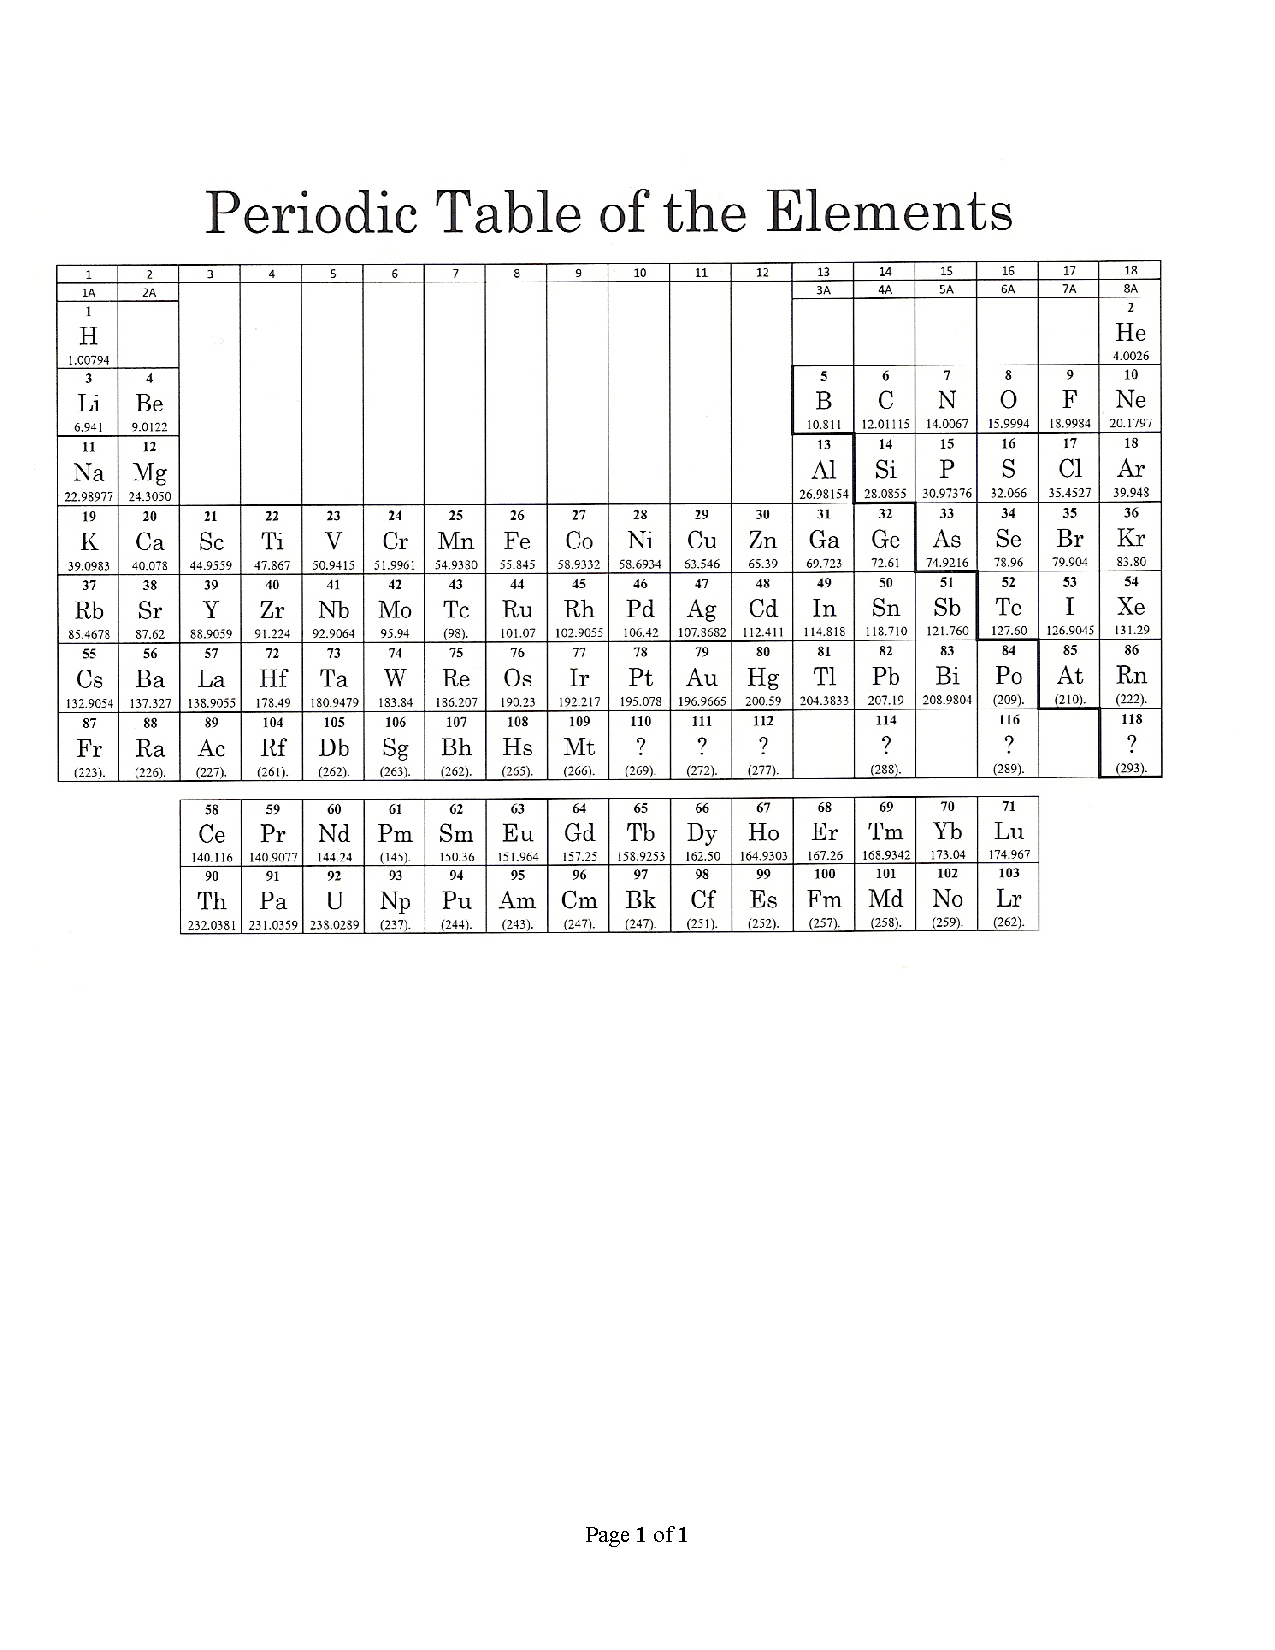
\includepdf[pages={-}]{Periodic Table for testing.pdf}

\end{document}